\scanpage{40}
\mspage{21}
Je vais expliciter les calculs dans le groupoïde $\mathrm{VII}$, associé au graphe de $=$ nom, on a des flèches génératrices
\[
(71)\qquad\left\{\begin{aligned}
\widetilde d_i^\omega&:P^\omega\longrightarrow R_i^\omega\\
\widetilde d_i^{\prime\omega}&:P^\omega\longrightarrow R_i^{\omega'}\\
a_i^\omega&:R_i^\omega\mathbin{-}R_i^{\omega'}
\end{aligned}\right.
\]
liées par les relations
\[
(72)\qquad\left\{\begin{aligned}
(\widetilde d_i^{\unsure{\omega\prime|\prime\omega}})^{-1}a_i^\omega\widetilde d_i^\omega&=1\\
(d_{\omega i}^{\prime\omega})^{-1}\widetilde d_{\omega i}^{\omega'}(d_i^{\prime\omega'})^{-1}\widetilde d_i^\omega&=1
\end{aligned}\right.
\]
\margin{six relations indépendantes exprimant les $\widetilde d_i^{\prime\omega}$ en termes des $\widetilde d_i^\omega$ et $a_i^\omega$, \inserted{ou les $\unsure{a_i^\omega}$ en termes des $\widetilde d_i^\omega,\widetilde d_i^{\prime\omega}$.}}
\margin{en apparence six relations, mais il n'y en a que trois indépendantes, car l'équation pour $i,\omega$ et pour $(\unsure{\omega i|i},\omega')$ est la $=$.}
\figure{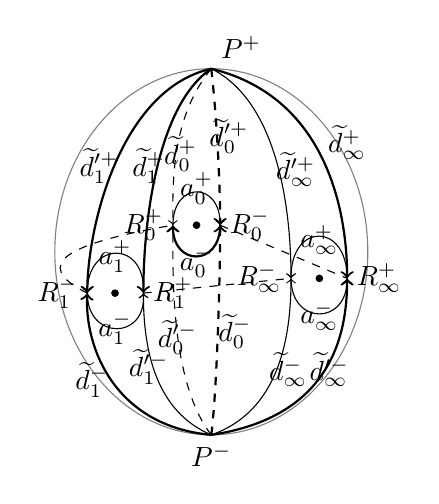
\begin{tikzpicture}[scale=.75]
\draw[gray] (0,0) ellipse (2.65 and 3.1);
\coordinate (P) at (0,3.1);\coordinate (M) at (0,-3.1);
\coordinate (L1) at (-2.1,-.7);\coordinate (R1) at (-1.15,-.7);
\coordinate (L0) at (-.65,.45);\coordinate (R0) at (.15,.45);
\coordinate (LI) at (1.35,-.45);\coordinate (RI) at (2.3,-.45);
\draw[dashed] (L1)..controls (-3.1,-.2) and (-2.4,.15)..(L0);
\draw[dashed] (R0)--(RI);\draw[dashed] (R1)--(LI);
\fill (-1.63,-.7) circle (.065);\fill (-.25,.45) circle (.065);\fill (1.83,-.45) circle (.065);
\draw[->,thick] (P)..controls (-1.55,2.75) and (-2.1,.4)..(L1);
\draw[->,thick] (P)..controls (-.9,2.5) and (-1.15,.55)..(R1);
\draw[dashed,->] (P)..controls (-.7,2.25) and (-.65,1.1)..(L0);
\draw[dashed,->,thick] (P)..controls (.1,2.2) and (.15,1.1)..(R0);
\draw[->] (P)..controls (1.2,2.5) and (1.35,.5)..(LI);
\draw[->,thick] (P)..controls (2.05,2.6) and (2.3,.5)..(RI);
\draw[->,thick] (M)..controls (-1.65,-2.95) and (-2.15,-1.6)..(L1);
\draw[->] (M)..controls (-.95,-2.7) and (-1.15,-1.65)..(R1);
\draw[dashed,->] (M)..controls (-.7,-2.2) and (-.65,-.35)..(L0);
\draw[dashed,->,thick] (M)..controls (.1,-2.3) and (.15,-.35)..(R0);
\draw[->] (M)..controls (1.15,-2.7) and (1.35,-1.45)..(LI);
\draw[->,thick] (M)..controls (2,-2.8) and (2.3,-1.45)..(RI);
\draw[->] (R1)..controls (-1.1,.2) and (-2.1,.2)..(L1);
\draw[->] (L1)..controls (-2.1,-1.5) and (-1.1,-1.5)..(R1);
\draw[->] (L0)..controls (-.65,1.2) and (.15,1.2)..(R0);
\draw[->,thick] (R0)..controls (.15,-.25) and (-.65,-.25)..(L0);
\draw[->] (RI)..controls (2.3,.5) and (1.35,.5)..(LI);
\draw[->] (LI)..controls (1.35,-1.25) and (2.3,-1.25)..(RI);
\node[above right] at (P) {$P^+$};\node[below] at (M) {$P^-$};
\node[left] at (L1) {$R_1^-$};\node[right] at (R1) {$R_1^+$};
\node[left] at (L0) {$R_0^+$};\node[right] at (R0) {$R_0^-$};
\node[left] at (LI) {$R_\infty^-$};\node[right] at (RI) {$R_\infty^+$};
\node at (-1.63,-.08) {$a_1^+$};\node at (-1.63,-1.3) {$a_1^-$};
\node at (-.25,1.07) {$a_0^+$};\node at (-.25,-.17) {$a_0^-$};
\node at (1.83,.2) {$a_\infty^+$};\node at (1.83,-1.08) {$a_\infty^-$};
\node at (-1.9,1.45) {$\widetilde d_1^{\prime+}$};\node at (-1.06,1.45) {$\widetilde d_1^+$};
\node at (-.52,1.65) {$\widetilde d_0^+$};\node at (.3,1.95) {$\widetilde d_0^{\prime+}$};
\node at (1.43,1.4) {$\widetilde d_\infty^{\prime+}$};\node at (2.3,1.85) {$\widetilde d_\infty^+$};
\node at (-2.02,-2.17) {$\widetilde d_1^-$};\node at (-1.06,-1.95) {$\widetilde d_1^{\prime-}$};
\node at (-.57,-1.45) {$\widetilde d_0^{\prime-}$};\node at (.4,-1.35) {$\widetilde d_0^-$};
\node at (1.3,-2) {$\widetilde d_\infty^-$};\node at (2,-2) {$\widetilde d_\infty^{\prime-}$};
\end{tikzpicture}}
On va repérer $u$ par les équations
\[
(73)\qquad\left\{\begin{aligned}
u(\widetilde d_i^\omega)&=\deleted{\unsure{\widetilde d_i^\omega}}\varphi_i^\omega(\xi_1^{\deleted{\unsure{'}}})\widetilde d_i^\omega\\
u(\widetilde d_i^{\prime\omega})&=\deleted{\unsure{\widetilde d_i^{\prime\omega}}}\varphi_i^{\omega'}(\xi')\widetilde d_i^{\prime\omega}\\
u(a_i^\omega)&=a_i^\omega\varphi_i^\omega(\lambda)
\end{aligned}\right.\qquad \xi',\xi_1^{\deleted{\unsure{'}}},\lambda\in\widehat\Pi_{0,3}
\]
et il reste à exprimer que $u$ satisfait les relations (72). La première s'explicite sous la forme
\[
(74)\qquad\xi'=\varepsilon_0(\lambda\xi_1)\qquad\text{i.e.}\quad\xi_1=\lambda^{-1}\cdot\varepsilon_0^{-1}(\xi')
\]
et on trouve également
\[
(75)\qquad\deleted{\unsure{\beta}}\xi_1=\beta'\sigma_\infty(\xi')
\]
\margin{où $\beta'$ défini par la condition $(\unsure{65\,a|65\,'})$}
Cette \unsure{relation|relations} permettant de tirer $\beta'$ en termes
\margin{39}
